\usetikzlibrary{arrows.meta,calc}

\tikzset{
    >=Latex,
}

\begin{frame}{individual computers are networks}
\begin{itemize}
    \item individual computers are (kinda) networks of\ldots
    \begin{itemize}
        \item processors
        \item memories
        \item I/O devices
    \end{itemize}
    \vspace{.5cm}
    \item so what topology (layout) do those networks have?
    \end{itemize}
\end{frame}

\begin{frame}{the ``bus'' (1)}
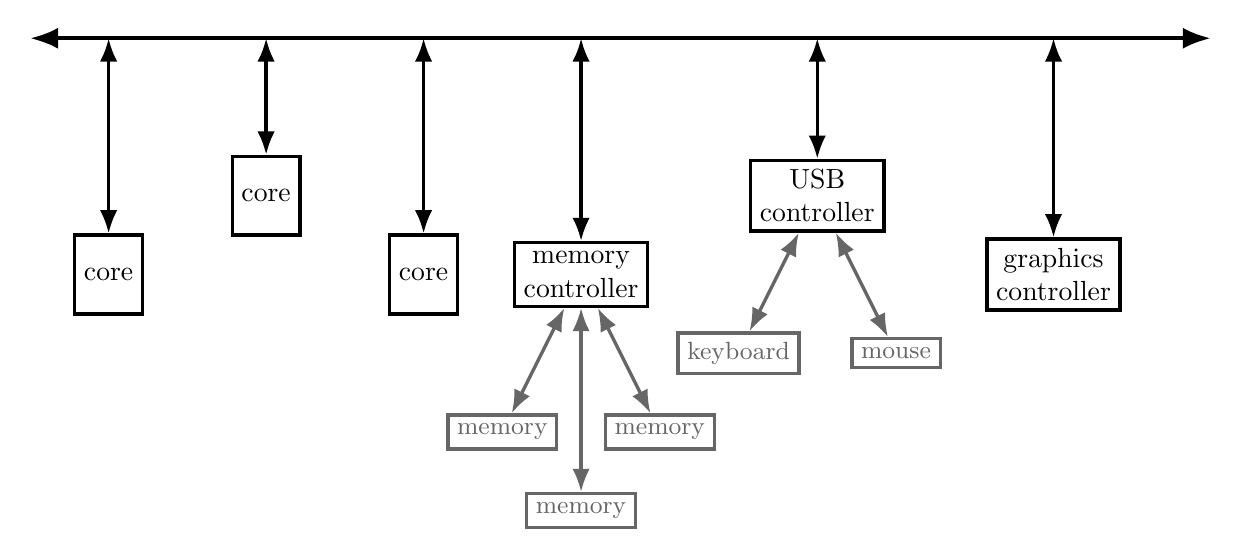
\begin{tikzpicture}
\draw[ultra thick,<->] (0, 0) -- (15, 0);
\node[draw,very thick,align=center,minimum height=1cm] (core 1) at (1, -3) {core};
\node[draw,very thick,align=center,minimum height=1cm] (core 2) at (3, -2) {core};
\node[draw,very thick,align=center,minimum height=1cm] (core 3) at (5, -3) {core};
\node[draw,very thick,align=center] (memory) at (7, -3) {memory\\controller};
\node[draw,very thick,align=center] (usb) at (10, -2) {USB\\controller};
\node[draw,very thick,align=center] (graphics) at (13, -3) {graphics\\controller};
\node[font=\small,draw,black!60,very thick,align=center] (memory chip 1) at (6, -5) {memory};
\node[font=\small,draw,black!60,very thick,align=center] (memory chip 2) at (7, -6) {memory};
\node[font=\small,draw,black!60,very thick,align=center] (memory chip 3) at (8, -5) {memory};
\foreach \x in {1,2,3} {
    \draw[black!60,very thick,<->] (memory chip \x) -- (memory);
}
\node[font=\small,draw,black!60,very thick,align=center] (usb 1) at (9, -4) {keyboard};
\node[font=\small,draw,black!60,very thick,align=center] (usb 3) at (11, -4) {mouse};
\foreach \x in {1,3} {
    \draw[black!60,very thick,<->] (usb \x) -- (usb);
}
\foreach \x in {core 1,core 2,core 3,memory,usb,graphics} {
    \draw[<->,very thick] (\x) -- (0,0 -| \x);
}
\end{tikzpicture}
\end{frame}

% FIXME: Intel 80386 block diagram as comparison


\begin{frame}{example: 80386 signal pins}
\begin{tabular}{|l|l|l|}
\hline
\bfseries name & \multicolumn{2}{|l|}{\bfseries purpose} \\ \hline 
CLK2 & clock for bus & timing\\ \hline
W/R\# & write or read? & \multirow{4}{*}{metadata} \\ \cline{1-2}
D/C\# & data or control? &~ \\ \cline{1-2}
M/IO\# & memory or I/O? &~\\ \cline{1-2}
INTR & interrupt request &~\\ \cline{1-2}
\ldots & other metadata signals &~\\ \hline
BE0\#-BE3\# & (4) byte enable & \multirow{2}{*}{address} \\\cline{1-2}
A2-A31 & (30) address bits &~\\ \hline
DO-D31 & (32) data signals & data\\ \hline
\end{tabular}
\imagecredit{adapted from the Intel 80386 Hardware Reference Manual (1986)}
\end{frame}

\begin{frame}{example: AMD EPYC (1 socket)}
\includegraphics[height=0.9\textheight]{../buses/zepplin-fig21}
\imagecredit{Figure from Burd et al,  \\ `` `Zepllin': An SoC for Multichip Architectures'' (IEEE JSSC Vol 54, No 1)}
\end{frame}

\begin{frame}{example: Intel Skylake-SP}
\includegraphics[height=0.85\textheight]{../buses/skylake-mesh}
\imagecredit{Figure from Tam et al, ``SkyLake-SP: A 14nm 28-Core Xeon® Processor'' (ISSCC 2018)}
\end{frame}

% FIXME: recent AMD/Intel block diagram for network 
    % Intel Mesh network
    % 
